\documentclass{beamer}
\usetheme{Boadilla}
\usepackage{xcolor}
\usepackage{tikz}

\title{Cellular Automata}
\subtitle{An introduction to Conway's Game of Life}
\author{Aniruddha Deb}
\institute{IIT Delhi}
\date{\today}

\begin{document}

\begin{frame}
\titlepage
\end{frame}

\begin{frame}
\frametitle{Determinism and Non-Determinism}
\pause
\begin{flushleft}
A \textbf{Deterministic Algorithm} is an algorithm that repeatedly gives the
same set of outputs for a given set of outputs. An example is a simple function
$f(x) = x^2$
\end{flushleft}

\begin{center}
	\tikzset{every picture/.style={line width=0.75pt}} %set default line width to 0.75pt        
	
	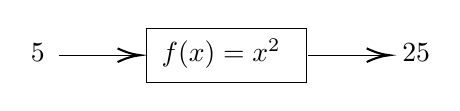
\begin{tikzpicture}[x=0.75pt,y=0.75pt,yscale=-1,xscale=1]
	
	%Shape: Rectangle [id:dp16197166944169683] 
	\draw   (221,80.97) -- (298,80.97) -- (298,106.97) -- (221,106.97) -- cycle ;
	%Straight Lines [id:da07695618334677845] 
	\draw    (179,93.97) -- (216,93.97) ;
	\draw [shift={(218,93.97)}, rotate = 180] [color={rgb, 255:red, 0; green, 0; blue, 0 }  ][line width=0.75]    (10.93,-3.29) .. controls (6.95,-1.4) and (3.31,-0.3) .. (0,0) .. controls (3.31,0.3) and (6.95,1.4) .. (10.93,3.29)   ;
	%Straight Lines [id:da47094111370416836] 
	\draw    (299,93.97) -- (336,93.97) ;
	\draw [shift={(338,93.97)}, rotate = 180] [color={rgb, 255:red, 0; green, 0; blue, 0 }  ][line width=0.75]    (10.93,-3.29) .. controls (6.95,-1.4) and (3.31,-0.3) .. (0,0) .. controls (3.31,0.3) and (6.95,1.4) .. (10.93,3.29)   ;
	
	% Text Node
	\draw (227,85) node [anchor=north west][inner sep=0.75pt]    {$f( x) =x^{2}$};
	% Text Node
	\draw (164,87) node [anchor=north west][inner sep=0.75pt]    {$5$};
	% Text Node
	\draw (343,87) node [anchor=north west][inner sep=0.75pt]    {$25$};
	\end{tikzpicture}
\end{center}

\pause
\begin{flushleft}
A \textbf{Nondeterministic Algorithm} is an algorithm that does not give 
repeatable outputs for a given input. An example is a cup in which n dice 
are rolled. ($g:\Bbb{N} \to \Bbb{N}^n$)
\end{flushleft}
\begin{center}
	\tikzset{every picture/.style={line width=0.75pt}} %set default line width to 0.75pt        
	
	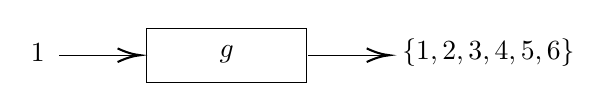
\begin{tikzpicture}[x=0.75pt,y=0.75pt,yscale=-1,xscale=1]
	
	%Shape: Rectangle [id:dp16197166944169683] 
	\draw   (221,80.97) -- (298,80.97) -- (298,106.97) -- (221,106.97) -- cycle ;
	%Straight Lines [id:da07695618334677845] 
	\draw    (179,93.97) -- (216,93.97) ;
	\draw [shift={(218,93.97)}, rotate = 180] [color={rgb, 255:red, 0; green, 0; blue, 0 }  ][line width=0.75]    (10.93,-3.29) .. controls (6.95,-1.4) and (3.31,-0.3) .. (0,0) .. controls (3.31,0.3) and (6.95,1.4) .. (10.93,3.29)   ;
	%Straight Lines [id:da47094111370416836] 
	\draw    (299,93.97) -- (336,93.97) ;
	\draw [shift={(338,93.97)}, rotate = 180] [color={rgb, 255:red, 0; green, 0; blue, 0 }  ][line width=0.75]    (10.93,-3.29) .. controls (6.95,-1.4) and (3.31,-0.3) .. (0,0) .. controls (3.31,0.3) and (6.95,1.4) .. (10.93,3.29)   ;
	
	% Text Node
	\draw (255,88) node [anchor=north west][inner sep=0.75pt]    {$g$};
	% Text Node
	\draw (164,87) node [anchor=north west][inner sep=0.75pt]    {$1$};
	% Text Node
	\draw (343,85) node [anchor=north west][inner sep=0.75pt]    {$\{1,2,3,4,5,6\}$};
	\end{tikzpicture}
\end{center}
\end{frame}

\begin{frame}
\frametitle{State Machines}
\pause
\begin{flushleft}
A \textbf{Finite State Machine} or \textbf{Finite State Automata} is a machine that can exist in exactly one of a finite
number of states at a given point in time, and can \textit{transition} between these states
as a result of inputs. A simple example is a switch.

\begin{center}
	\tikzset{every picture/.style={line width=0.75pt}} %set default line width to 0.75pt        
	
	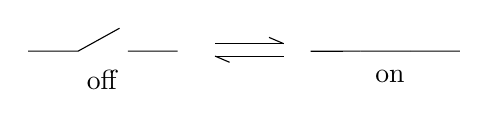
\begin{tikzpicture}[x=0.75pt,y=0.75pt,yscale=-1,xscale=1]
	%uncomment if require: \path (0,300); %set diagram left start at 0, and has height of 300
	
	%Straight Lines [id:da8818602134387576] 
	\draw    (14,20) -- (38,19.97) ;
	%Straight Lines [id:da6777788892413668] 
	\draw    (62,20) -- (86,19.97) ;
	%Straight Lines [id:da9797738416661963] 
	\draw    (38,20.03) -- (58,8.97) ;
	%Straight Lines [id:da978073320202391] 
	\draw    (150,20.05) -- (174,20.03) ;
	%Straight Lines [id:da7322212805692465] 
	\draw    (198,20) -- (222,19.97) ;
	%Straight Lines [id:da027703079406747655] 
	\draw    (174,20.03) -- (198,20) ;
	%Straight Lines [id:da7737672298064389] 
	\draw    (104,16.38) -- (137,16.38) ;
	%Straight Lines [id:da6321717459304543] 
	\draw    (104,22.38) -- (137,22.38) ;
	%Straight Lines [id:da0825108051498844] 
	\draw    (130,13.38) -- (137,16.38) ;
	%Straight Lines [id:da3024067774927739] 
	\draw    (104,22.38) -- (111,25.38) ;
	
	% Text Node
	\draw (41,27.97) node [anchor=north west][inner sep=0.75pt]   [align=left] {off};
	% Text Node
	\draw (180,27.97) node [anchor=north west][inner sep=0.75pt]   [align=left] {on};
	\end{tikzpicture}
\end{center}
\end{flushleft}
\pause
\begin{flushleft}
\textcolor{red}{Can we make an infinite state machine by combining infinite 
finite state machines?} \pause Theoretically yes, but practically no.
\end{flushleft}
\end{frame}

\begin{frame}
\frametitle{Deterministic and Nondeterministic Finite State Machines}
\begin{flushleft}
Combining both these concepts, a \textbf{Deterministic Finite State Automata (DFA)}
is one whose next state is uniquely determined by the current state
\end{flushleft}
\end{frame}

\end{document}
